\begin{theo}
Если функция $u(M)$, определённая и непрерывная в замкнутой области $T + \Sigma$, удовлетворяет уравнению $\Delta u = 0$ внутри $T$, то максимальные и минимальные значения функции достигаются на поверхности $\Sigma$ (\textbf{принцип максимального значения}).
\end{theo}
\begin{qproof}
Допустим, что функция $u(M)$ достигает максимального значения в некоторой внутренней точке $M_0$ области $T$, так что $u_0 = y(M_0) \geqslant u(M)$, где $M$ --- любая точка области $T$. Окружим точку $M_0$ сферой $\Sigma_\rho$ радиуса $\rho$, целиком лежащей внутри области $T$. Поскольку, по предположению, $u(M_0)$ есть наибольшее значение функции $u(M)$ в $T + \Sigma$, то $u|_\Sigma \leqslant u (M_0)$. Пользуясь формулой среднего значения 
\[
	u(M_0) = \frac{1}{4 \pi a^2} \iint\limits_{\Sigma_a} u \, d \sigma
\]
и заменяя под интегралом всюду $u(M)$ значением $u(M_0)$, получим:
\[
	u(M_0) = \frac{1}{4 \pi \rho^2} \iint\limits_{\Sigma_\rho} u(M)\, d\sigma_M \leqslant \frac{1}{4 \pi \rho^2} \iint\limits_{\Sigma_\rho} u (M_0) \, d \sigma = u(M_0).
\]
Если предположить, что хотя бы в одной точке $M$ сферы $\Sigma_\rho$ $u(M) M u(M_0)$, то очевидно, что вместо знака $\leqslant$ будем иметь знак $<$, что приводит к противоречию. Таким образом, на всей поверхности $\Sigma_\rho \quad u(M) \equiv u(M_0)$.

Если $\rho_0^m$ --- минимальное расстояние от $M_0$ до поверхности $\Sigma$, то $u(M) \equiv u(M_0)$ для всех точке, лежащих внутри $\Sigma_{\rho_0^m}$. Отсюда следует, что в точках $M^*$, принадлежащих общей части $\Sigma_{\rho_0^m}$ и $\Sigma$, по непрерывности $u(M^*) \equiv u(M_0)$. Это и доказывает теорему, поскольку мы убедились, что максимальное хначение $u(M_0)$ достигается в точках границы $M^*$.\\
\begin{figure}[h!]
	\centering
	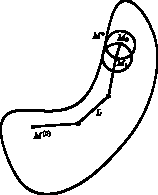
\includegraphics[scale=1.5]{figLaplaceMax.pdf}
\end{figure}

Нетрудно убедиться, что если область $T$ связная и максимальное значение достигается хотя бы в одной внутренней точке $M_0$, то $u(M) \equiv u(M_0)$ во всей области. Пусть $M^{(0)}$ --- какая-либо другая точка области $T$. Соединим точку $M^{(0)}$ с точкой $M_0$ ломаной линией $L$, длину которой обозначим $l$. Пусть $M_1$ есть последняя точка выхода линии $L$ из $\Sigma_{\rho^m}$. В этой точке $u(M_1) = u(M_0)$. Опишем из этой точки сферу $\Sigma_{\rho^m}$ радиуса $\rho_1^m$, касающуюся $\Sigma$, и пусть $M_2$ --- последняя точка выхода $L$ из $\Sigma_{\rho_1^m}$; в этой точке $u(M_2) = u(M_0)$. Продолжая этот процесс далее получим, что не более чем через $p = l / \rho^{(m)}$ шагов, где $\rho^{(m)}$ --- минимальное расстояние от $L$ до $\Sigma$, одна из этих сфер захватит точку $M^{(0)}$, откуда следует, что $u(M^{(0)}) = u (M_0)$. В силу произвольности $M^{(0)}$ и непрерывности $u(M)$ в замкнутой области $T + \Sigma$, заключаем, что $u(M) \equiv u (M_0)$ всюду, включая точки границы. Таким образом, из всех гармонических функций только постоянная может достигать своего максимального значения во внутренних точках области.
\end{qproof}
